%about objects not information; we can discuss in outside the box the issue of
%information needed forver but shuttled in and out.

\chapter{When It Won't Fit: Bulk Storage}
%\chapter{Extreme Scalability of Long-lived Data}
\label{chapter:large-long-lived}
\index{Bulk Storage}

% All of the tuning advice presented so far in this book can only get you so
% far.
There are limits to how well an object-oriented data model can scale.
At some point, you will be faced with the ineluctable limits of tuning objects.
Each object has its header, and this is an unavoidable cost. The only way to
avoid delegation costs, and thus amortize the cost of a header over more data
fields, is to go through the manual, iterative, process of inlining the fields
of one class into another. Some amount of this manual inlining makes sense, but
too much runs counter to principled engineering. Often, you are blocked because
you run into code that you do not own, or classes whose field layout is,
for one reason or another, set in stone.

In this way, a conventional storage strategy, one which maps entities to objects
and relations to collections, suffers from two problems that impact scaling up
the size and complexity of a design.

\paragraph{Amortizing away header costs.} Since entities are
  objects, and each object pays a header cost imposed by the \jre, you need to
  craft your design so that there is enough data in each object to amortize the
  cost of the headers, and to avoid high delegation costs.
 
\begin{wrapfigure}{r}{0.31\textwidth}
 \centering
 \vspace{-2mm}
 \begin{framedlisting}
 class X {
   A a;
 }
 class B extends A {
   int w, x;
 }
 class C extends A {
   int z;
 }
 \end{framedlisting}
 \caption{Delegation costs one object header, a cost that is easy to amortize.} 
 \label{fig:fragile-base-class}
\end{wrapfigure}
\paragraph{The Fragile Base Class problem.}
 %Any attempt to optimize, by
 %manually inlining the fields of one class into another, will likely suffer
 %from the fragile base class problem.
 \index{Fragile base class problem}
You may (wisely!) be unwilling to touch a class that is also used by other
 teams for fear of adversely impacting their correctness or
 memory footprint. For example, say class \class{X} delegates some of its
 behavior to an instance of class \class{A}, and that both \class{B} (your
 class) and \class{C} (the other team's class) are instances of \class{A}.
 %\autoref{fig:fragile-base-class} shows this example.
 Ignoring the other teams needs, you might prefer to collapse the fields of
 \class{B} into the \class{X} class, removing this need for delegation and that
 extra object header. To do so requires either modifying the implementation of
 \class{X}, or duplicating the implementation of \class{X} into a modified version of \class{B}. Neither alternative seems very appealing.
 This is a variant of what is known as the \emph{fragile base class problem}.

\begin{wrapfigure}{l}{0.47\textwidth}
\centering
   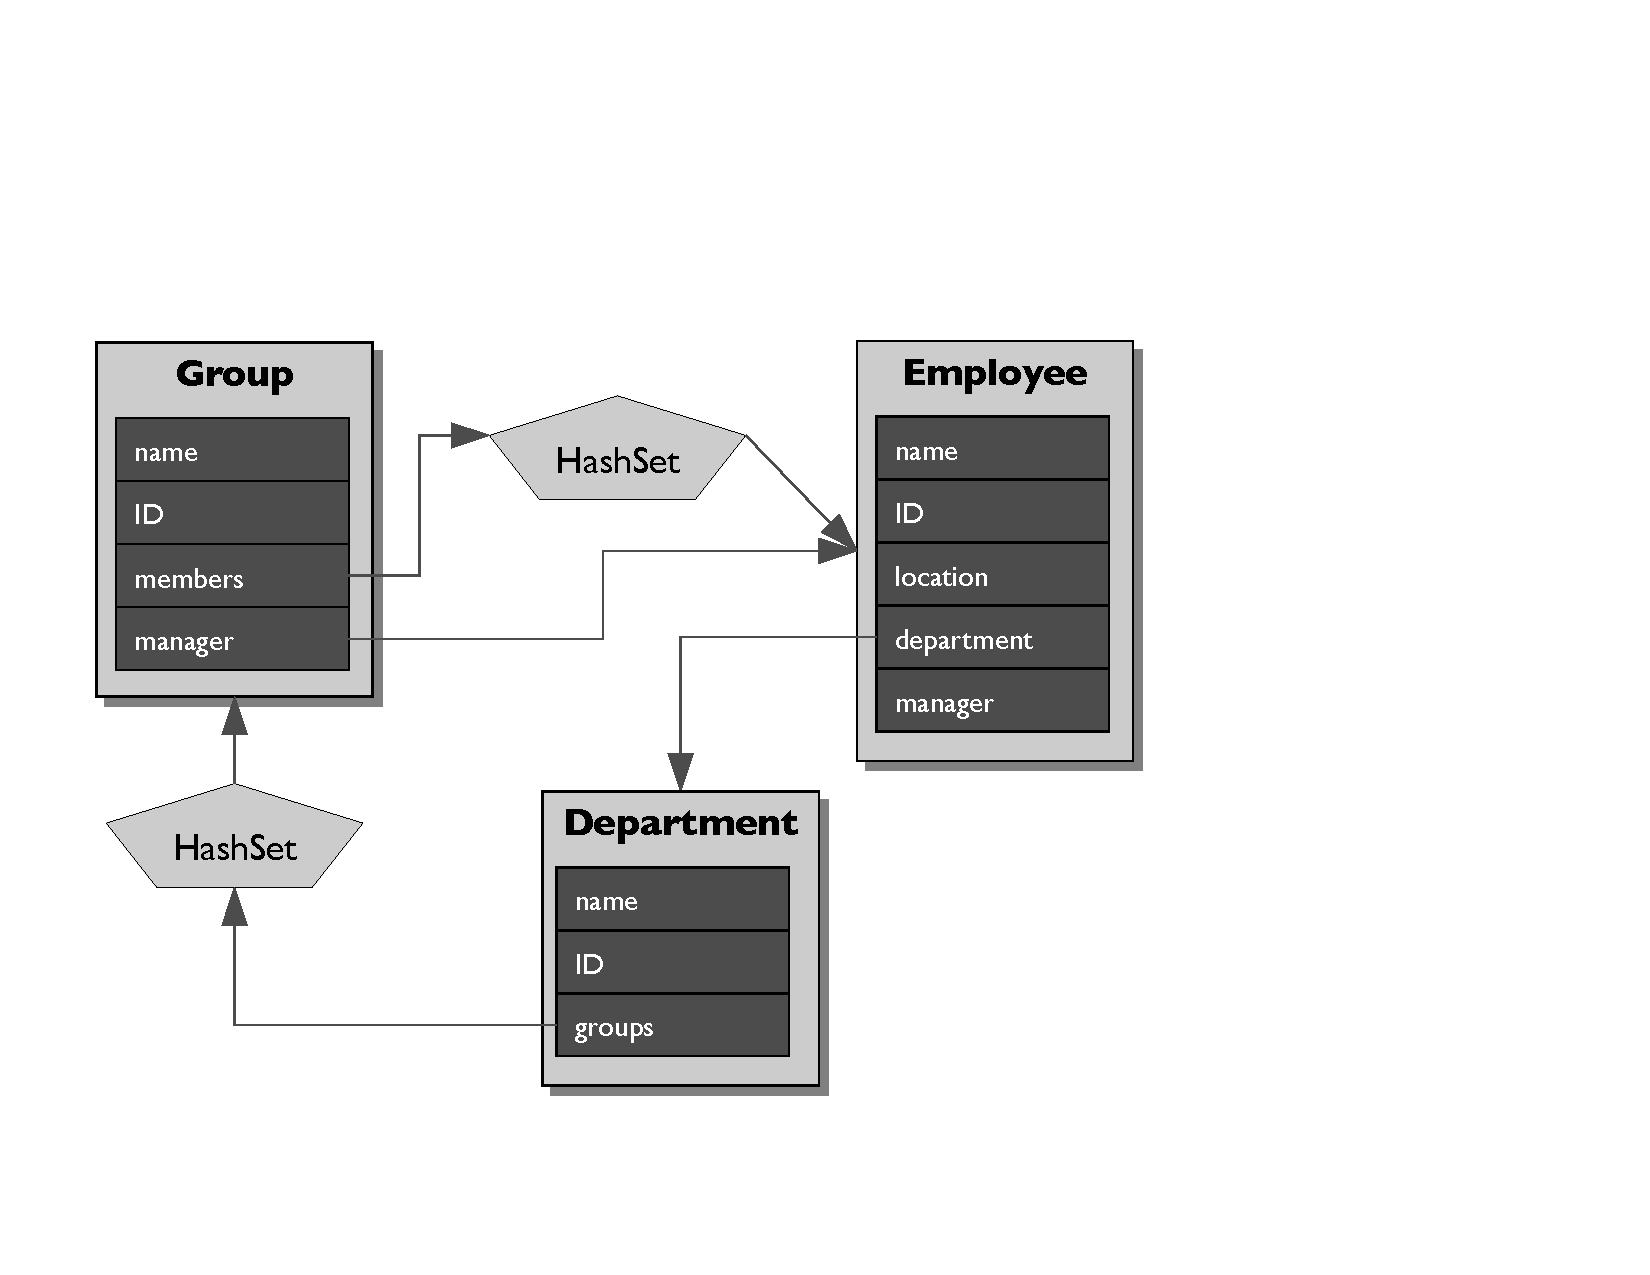
\includegraphics[width=0.46\textwidth]{part3/Figures/extreme/EC-example-for-columns1}
   \caption{A conventional storage strategy maps entities to objects, 
   attributes to fields, and relations to collections.}
   \label{fig:extreme-ec}
\end{wrapfigure}
If you break out of the Java mold, you can overcome these issues. An
Entity-Collection diagram such as \autoref{fig:extreme-ec} maps pretty
inefficiently to a straightforward Java implementation. Each entity pays a
header cost, but has only a few data fields. Most of the collections,
representing relationships such as the number of employees under a manager, will
be small. 

\begin{wrapfigure}[13]{l}{0.3\textwidth}
\centering
   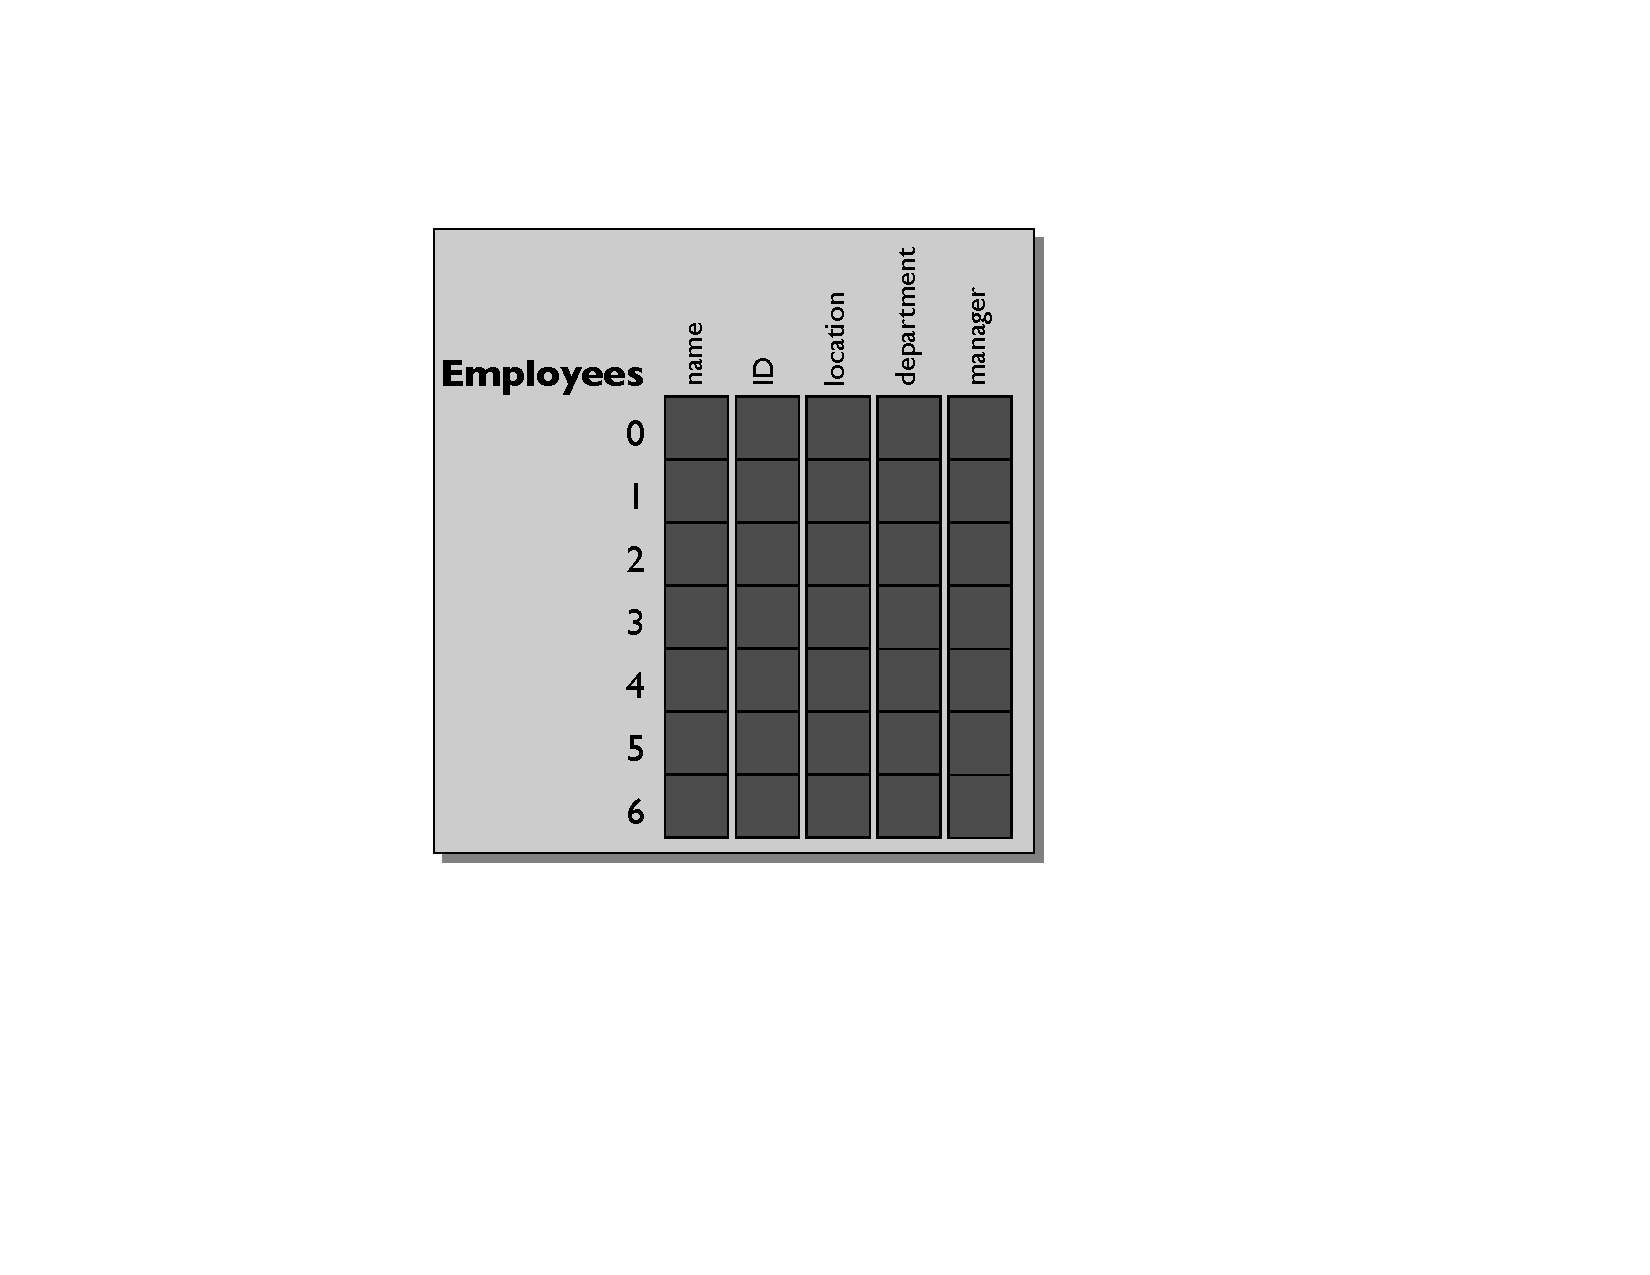
\includegraphics[width=0.28\textwidth]{part3/Figures/extreme/EC-example-for-columns2}
   \caption{With column-oriented storage, each attribute is stored in an array
   of pure data.}
\end{wrapfigure}

Storing data in bulk form means that the relations are stored in a small and
fixed number of collections, and the entities are stored in a small and fixed
number of objects --- across \emph{all} entities and relations between them.
They key is that the number of allocations is small and fixed, and therefore
object header overheads (and allocation costs) are easily amortized. The trick
to accomplishing a bulk storage approach is to store data in large arrays. This
can be accomplished in two ways: arrays of records and column-oriented storage.
Arrays of records are not an option in Java, and so this chapter focuses on the
latter approach.

In a way that a graph of interconnected Java objects can never be, this bulk
approach of storage is highly optimized for having a large number of entities.
However, you must not forget that bulk storage violates some basic tenets of
object-oriented data modeling. These benefits to scalability come with some
design costs, and may not suit the way your data is accessed and updated.
Nonetheless, with careful consideration of these issues, you can reap
substantial benefits.



%Sometimes, despite your best effors of tuning entities and collections, your
%application's objects still do not fit into the memory constraints of the
%target platform. 


%Managing a great number of long-lived objects therefore comes with its
%own set of challenges, even though objects these objects are free from the bugs
%that riddle those with correlated lifetime. To manage objects that, after a
%reasonable amount of tuning, still don't fit into the heap, you have three
%solutions at your disposal: throw hardware at the problem, implement a kind of
%demand paging, or code your data models in a non-object oriented way.


\section{When to Consider Using Bulk Storage}

also, the data doesn't need to be long-lived, that's an (also imprecise)
description of the preconditions under which the technique (bulk storage)
applies. it's also not read-mostly, because, with bulk storage, it's ok if the
attribute values change rapidly (in fact, things will probably be faster here,
due to cache locality), and it's also ok if the set of attributes changes (here
again bulk storage does a better job, much better in this case, than java). the
only thing that can't happen too much is deletion of entities.

3(you wrote, in your notes, "Is the data immutable", and "is it stable after a
point in time", neither of which is i think an absolute precondition of bulk
storage, or at least not that broadly; immutability only matters for the domain
of entities, but, even then, additions are OK, and even infrequent removals are
OK; or is this what you meant by "stability"?)

\section{A Bulk Storage Strategy: Column-oriented Storage}
\label{sec:column-oriented}
\index{Column-oriented Storage}

The examples of the previous section worked through various optimizations of
representing relationships, and illustrated the interplay of storage optimization
and API design. Very often, achieving a high level of memory efficiency requires
breaking what would generally considered to be the object orientation of the API
or the storage. The main goals are to support a combination of flexibility and
scalability that is not possible when following the precepts of object
orientation.

It would be nice if you could avoid the overhead of collections, without having
to pollute your code with special cases. It would also be nice if you could add
edge or node properties, without having to worry about the interaction of their
storage with the storage of the relations themselves. If your main use of the
relational information is for traversals that don't modify the graph structure
itself, then there is an opportunity to dramatically reduce the overheads of
storing this information.

\paragraph{Breaking the Mold of Object Orientation}

Consider the simple example graph from
\autoref{fig:example-storing-relations-graph}, which has been updated in
\autoref{fig:example-storing-relations-graph-with-node-numbers} to include a
dense index for each node. The indices are natural numbers that range, in this
example from 1--9, with no gaps. If each node has a dense index, then each node
attributes can be stored in a flattened form. If you store the data compactly,
you can avoid much of the pointer and header overhead that plagues most normal
object oriented storage representations.

\begin{wrapfigure}{l}{0.29\textwidth}
\begin{framedlisting}
struct Node {
   Color color;
}
struct Node[] nodes;
\end{framedlisting}
\caption{In C, you can use arrays of records.}
\end{wrapfigure}
\index{Fortran}
\index{COBOL}
\index{Pascal}
\index{Arrays of records}
To store data compactly, you have two options: either use arrays of records, or
in parallel arrays of attributes.

 either store data in the style of
C, Pascal, or COBOL arrays of records, or in the style of Fortran parallel
arrays. An array of C structs, or Pascal records, stores the fields of the structures
densely. The fields of each record are stored back to back in the array, without
intervening pointers or headers. 
%If the records of nodes are stored in
%an array called \code{nodes}, then
%to retrieve the color of the node
%with index 5 becomes \code{nodes[5].color}.

Unfortunately, Java does not allow for arrays of structures. If the storage size
of every field is known, and fixed, you can mimic this storage structure in Java,
to a point. However, if your records have fields of varying types, this style of
programming can boils down to doing the very same work you would do for
marshalling data in and out of the Java heap. If the first and third attributes
of your nodes are of \class{byte} size and the second is of \class{int} size,
then accessing the third field of the node with index 5 is tricky. It requires
treating the entire record as a bit bucket, and shifting and masking
appropriately.

\newcommand{\light}[1]{\footnotesize{\textcolor{Lighter}{#1}}}

\begin{wrapfigure}{r}{0.48\textwidth}
\begin{framedlisting}
class NodeModel {
  Color[] colors;
  Color getColor(int nodeIndex) {
    return colors[nodeIndex];
  }
}
\end{framedlisting}
\end{wrapfigure}
%\index{Fortran}
\index{Parallel arrays}
The alternative is to store your data in a column-oriented style, where each
attribute is stored in its own array. With this storage structure, you avoid the messy details
of addressing fields with a non-uniformly typed record. Furthermore, adding new
attributes to nodes or edges is a trivial operation. Each is merely an extra
array in the set of parallel arrays.
In this style of storage, you express
collections of objects, rather than individual objects. The individuals are
represented by indices. Instead of having a class for a node, you have a class
for a group of nodes that participate, together, in a graph or several related
graphs, as shown on the right.
\autoref{fig:fortran-style} gives an example of a graph with 9 nodes.

\begin{figure}
\centering
\subfigure[Example graph, where each node has been assigned a dense integer
index.]{
\label{fig:example-storing-relations-graph-with-node-numbers}
	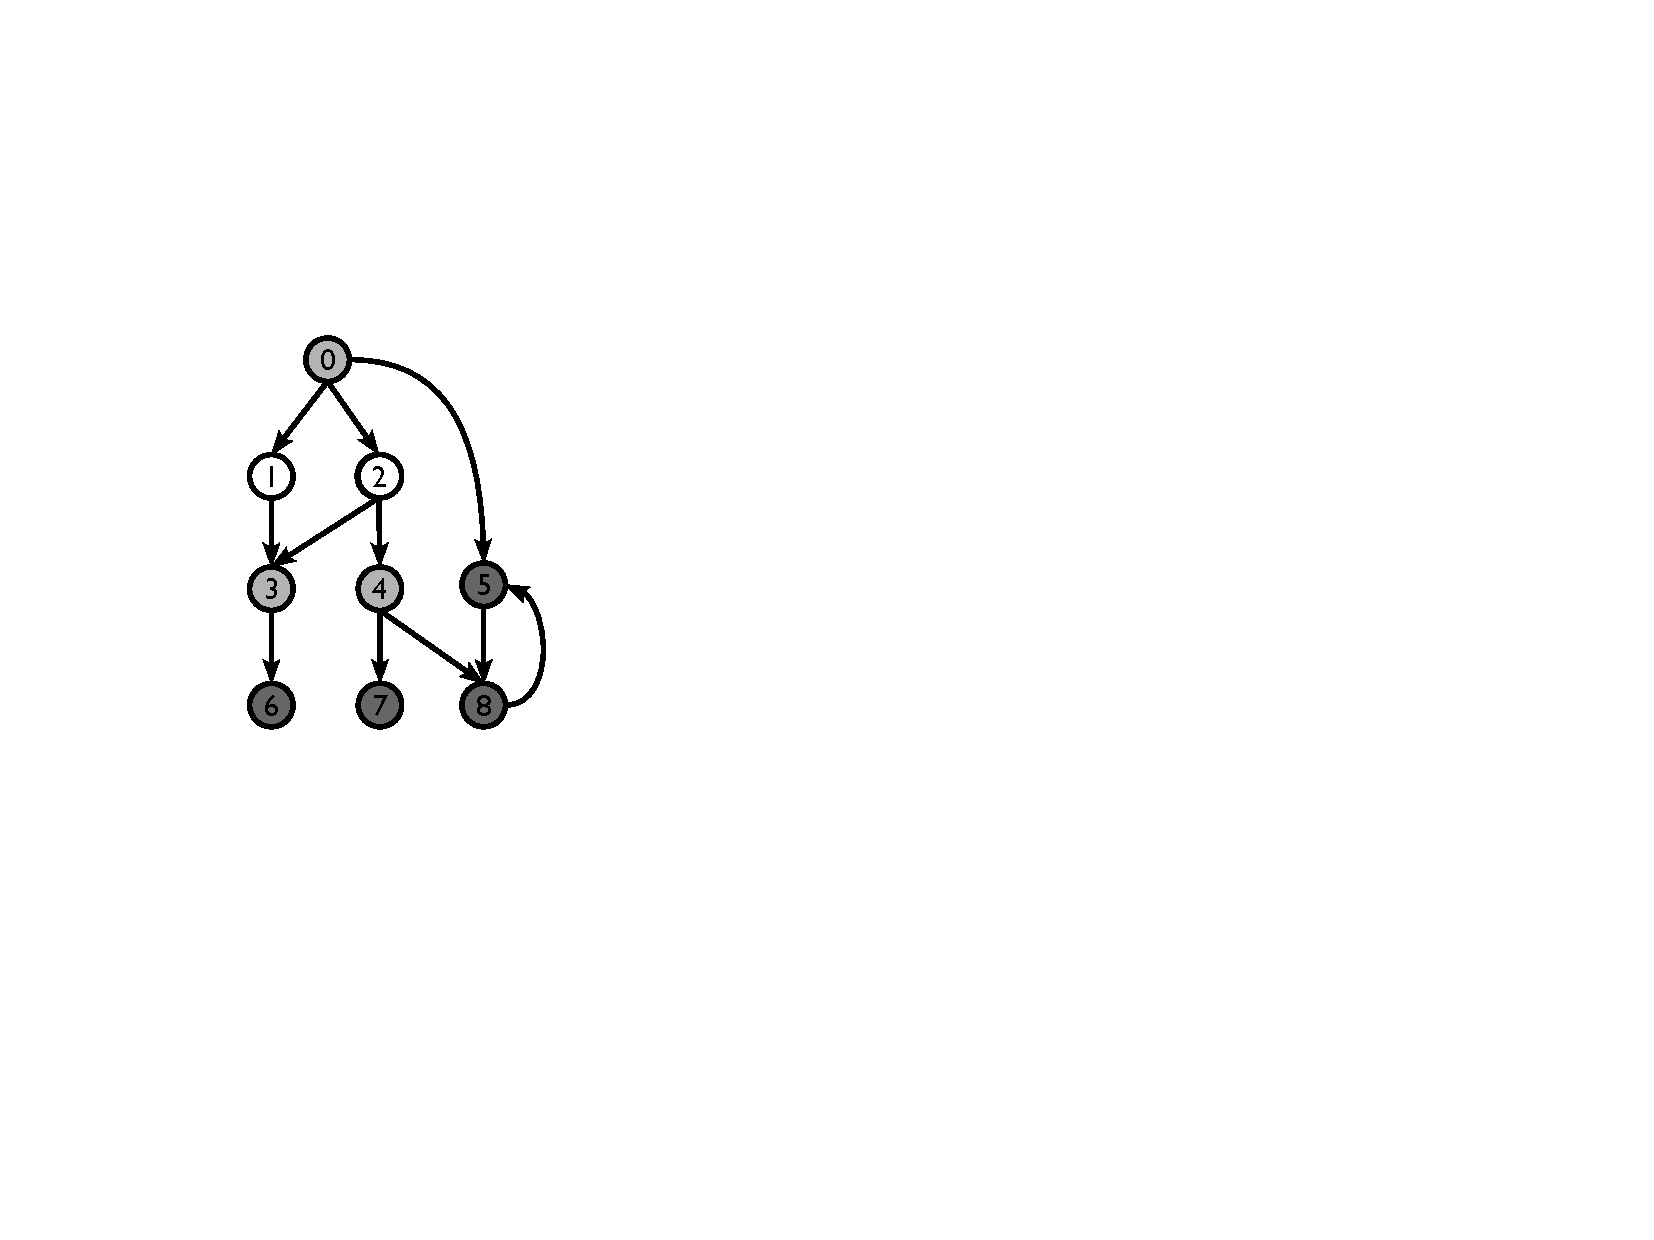
\includegraphics[width=0.3\textwidth]{part3/Figures/assessing/exampleGraph-withNodeNumbers}
	}
\quad
\subfigure[The node attribute.]{
\shortstack{
\begin{tabular}{ll}
\multicolumn{1}{r}{\light{index}} & \multicolumn{1}{l}{\textbf{Color}}
\\ \toprule
\light{0} & LightGray \\ \midrule
\light{1} & White \\ \midrule
\light{2} & White \\ \midrule
\light{3} & LightGray \\ \midrule
\light{4} & LightGray \\ \midrule
\light{5} & DarkGray \\ \midrule
\light{6} & DarkGray \\ \midrule
\light{7} & DarkGray \\ \midrule
\light{8} & DarkGray \\
\bottomrule
\end{tabular}
\\ \vspace{0mm}
}
}
\quad
\subfigure[Edges.]{
\shortstack{
\begin{tabular}{r@{~~$\rightarrow$~~}l}
\textbf{from} & \textbf{to}
\\ \toprule
0 & 1 \\
0 & 2 \\
0 & 5 \\ \midrule
1 & 3 \\ \midrule
2 & 3 \\
2 & 4 \\ \midrule
3 & 6 \\ \midrule
4 & 7 \\
4 & 8 \\ \midrule
5 & 8 \\ \midrule
8 & 5 \\
\bottomrule
\end{tabular}
\\ \vspace{0mm}
}
}
\caption{A graph of nodes and edges can be represented
as a set of parallel arrays --- a column-oriented approach to storage, in the
style of Fortran. Edge attributes, along with additional node attributes, would
be stored in additional columns. The \light{index} column is not a stored
attribute, it is only shown in the table, for clarity.}
\label{fig:fortran-style}
\end{figure}

If you need the convenience of an actual \class{Node} object, you can have a
bit of both worlds. As long as you use the node objects
only for temporary purposes, then you have a good chance of avoiding a memory
footprint problem. These transient node objects act as facades to the
\class{NodeModel}, but require a reference to the \class{NodeModel} and the
node's index. 
\begin{shortlisting}
class TransientNode {
   NodeModel nodeModel;
   int nodeIndex;
   Color getColor() {
      return nodeModel.getColor(nodeIndex);
   }
}
\end{shortlisting}
Though it has one extra field, on top of the earlier node implementations, for
the \class{NodeModel} reference, as long as it is transient, it could be fine.
This is something that requires experimentation in your setup. With transient
node facades, you are trading off more time spent in garbage collection for
convenience and the greater assurances you get from strong typing, compared to
passing around integers throughout your code, to represent node indices.
If these result in big drags in performance for your use cases, remember
that there is no absolute need for these transient node facades. You must also
be careful to either disallow, by convention, reference equality checks against
transient nodes, or cache any created objects.

The edges of a graph can be represented as two parallel arrays, storing the
source and target node indices of each edge, as shown in
\autoref{fig:fortran-style}c, and prototyped here:
\begin{shortlisting}
class EdgeModel {
   int[] from, to;
   int getEdgeFrom(int i) {
      return from[i];
   }
   int getEdgeTo(int i) {
      return to[i];
   }
}
\end{shortlisting}
However, this edge representation cannot efficiently support graph
traversals. There is no efficient way to retrieve the outgoing or
incoming edges from a given node. Even a \class{TransientEdge} class would not
help, because there is no connection between a node index and an index
into the edge model. Properly representing edges requires a bit more work. 

\section{Bulk Storage of Relationships}

To allow for efficient traversals of the edges, you must index them, as a
database would. First, consider the outgoing edges from a node. If the
\class{EdgeModel} parallel arrays are sorted by the \textbf{from} attribute, then
all of the children of a node will be stored contiguously. For example, the
edges in \autoref{fig:fortran-style}c have been sorted in this fashion.
At this point, it is
easy to establish an index, as an extra attribute of the \class{NodeModel}. This
attribute will store an index into this sorted edge model, which marks where the
children of each node begin. Once you have this index, then you no longer need to
store the \textbf{from} attribute in the edge model; it is implicit, in the
combination of the edge-start attribute of the node model. If you do so,
however, then you must also store the number of children of each node. 
\autoref{fig:fortran-style-edge-optimization} shows an update to
\autoref{fig:fortran-style}, where the node model now has, for the outgoing
edges, two new attributes: \textbf{EdgeStart} and \textbf{Num}. The same thing
can be done for the incoming edges, if we instead sort the edges of 
\autoref{fig:fortran-style}c by the \textbf{to} attribute.
\autoref{fig:fortran-style-edge-optimization}a also shows the two new attributes
for the incoming edges.  For example, node 2 has two children and
one parent. The children start at index 4 in
\autoref{fig:fortran-style-edge-optimization}b, which shows the two children to
be nodes 3 and 4.

\begin{figure}
\centering
\subfigure[Node attributes.]{
\shortstack{
\begin{tabular}{ll|ll|ll}
& & \multicolumn{2}{c|}{\textbf{Children}} &
\multicolumn{2}{c}{\textbf{Parents}} \\
\light{index} & \multicolumn{1}{l|}{\textbf{Color}} &
\multicolumn{1}{l}{\textbf{EdgeIndex}} & \multicolumn{1}{l|}{\textbf{Num}} & 
\multicolumn{1}{l}{\textbf{EdgeIndex}} &
\multicolumn{1}{l}{\textbf{Num}} \\ \toprule
\light{0} & LightGray & 0  & 3 & -- & 0 \\
\light{1} & White     & 3  & 1 & 0  & 1 \\
\light{2} & White     & 4  & 2 & 1  & 1 \\
\light{3} & LightGray & 6  & 1 & 2  & 2 \\
\light{4} & LightGray & 7  & 2 & 4  & 1 \\
\light{5} & DarkGray  & 9  & 1 & 5  & 2 \\
\light{6} & DarkGray  & -- & 0 & 7  & 1 \\
\light{7} & DarkGray  & -- & 0 & 8  & 1 \\
\light{8} & DarkGray  & 10 & 1 & 9  & 2 \\
\bottomrule
\end{tabular}
\\ \vspace{0mm}
}
}
\quad
\subfigure[Children edges.]{
\shortstack{
\begin{tabular}{ll}
\multicolumn{1}{r}{\light{index}} &
\multicolumn{1}{l}{\textbf{NodeIndex}} \\ \toprule
\light{0} & 1 \\
\light{1} & 2 \\
\light{2} & 5 \\ \midrule
\light{3} & 3 \\ \midrule
\light{4} & 3 \\
\light{5} & 4 \\ \midrule
\light{6} & 6 \\ \midrule
\light{7} & 7 \\
\light{8} & 8 \\ \midrule
\light{9} & 8 \\ \midrule
\light{10} & 5 \\
\bottomrule
\end{tabular}
\\ \vspace{0mm}
}
}
\quad
\subfigure[Parent edges.]{
\shortstack{
\begin{tabular}{ll}
\multicolumn{1}{r}{\light{index}} &
\multicolumn{1}{l}{\textbf{NodeIndex}}
\\ \toprule
\light{0} & 0 \\ \midrule  % 1 -> 0
\light{1} & 0 \\ \midrule  % 2 -> 0
\light{2} & 1 \\           % 3 -> 1
\light{3} & 2 \\ \midrule  % 3 -> 2
\light{4} & 2 \\ \midrule  % 4 -> 2
\light{5} & 0 \\ \midrule  % 5 -> 0
\light{6} & 8 \\           % 5 -> 8
\light{7} & 3 \\ \midrule  % 6 -> 3
\light{8} & 4 \\ \midrule  % 7 -> 4
\light{9} & 4 \\ \midrule  % 8 -> 4
\light{10} & 5 \\           % 8 -> 5
\bottomrule
\end{tabular}
\\ \vspace{0mm}
}
}
\caption{In order to support efficient traversal of the graph edges, you will
need to index them. These tables update the example of
\autoref{fig:fortran-style} to do so.  For example, node 2 has two children and
one parent. The children start at index 4 in
\autoref{fig:fortran-style-edge-optimization}b, which shows the two children to
be nodes 3 and 4.}
\label{fig:fortran-style-edge-optimization}
\end{figure}

%  used to have immutable in it
\section{Bulk Storage of Variable-length Data} %(e.g. Strings)}
\label{sec:bulk-sharing-pool}
\index{Bulk Sharing Pool}

Primitive arrays are often the repository for most of your application's actual
data. If your application has a few large primitive arrays, then the overhead of
the arrays will be dwarfed by the actual data contained therein. A common problem
with Java applications is that they have many small primitive arrays.
\index{Small Primitive Arrays} If the large majority of your actual data is in
these primitive arrays, and the average length of each array is 10 characters,
then your application will have a memory bloat factor of 61\%
% 16/(10 + 16)
--- almost half of your heap will be wasted on the object headers of the
primitive arrays. The problem grows worse if these primitive arrays are wrapped
inside of objects such as \class{String} or \class{ByteArrayOutputStream}. If
wrapped inside of \class{String} objects, then your application is doomed to a
memory bloat factor of 83\%.
% (16+32)/(10+16+32)

If these primitive arrays store only a small number of distinct sequences, this
problem of high overhead can, at least indirectly, be addressed by
interning.\index{Interning} Earlier, \autoref{sec:sharing-strings} discussed
string interning. If your primitive data is string data, then you can use the
\jres built-in mechansm for pooling this data, so that only one copy of each
string is kept in memory. For non-string data, you will have to roll your own
solution. In any case, however, interning only tackles a part of the problem at
hand. By keeping only a single canonical copy of the primitive data, you
eliminate the primitive array headers for the duplicates.
\autoref{fig:bulk-sharing-pool}(a) and \autoref{fig:bulk-sharing-pool}(b)
illustrate a simple case of interning. Of three strings, there are two duplicate
``grape'' sequences. The residual high overhead is due to the remaining
primitive array object headers; all of the \class{String} objects are eliminated
by interning. Interning removes only the primitive array overheads of
\emph{duplicate} strings.


\begin{figure}
\centering
	\subfigure[Three normal	\class{Strings}.]{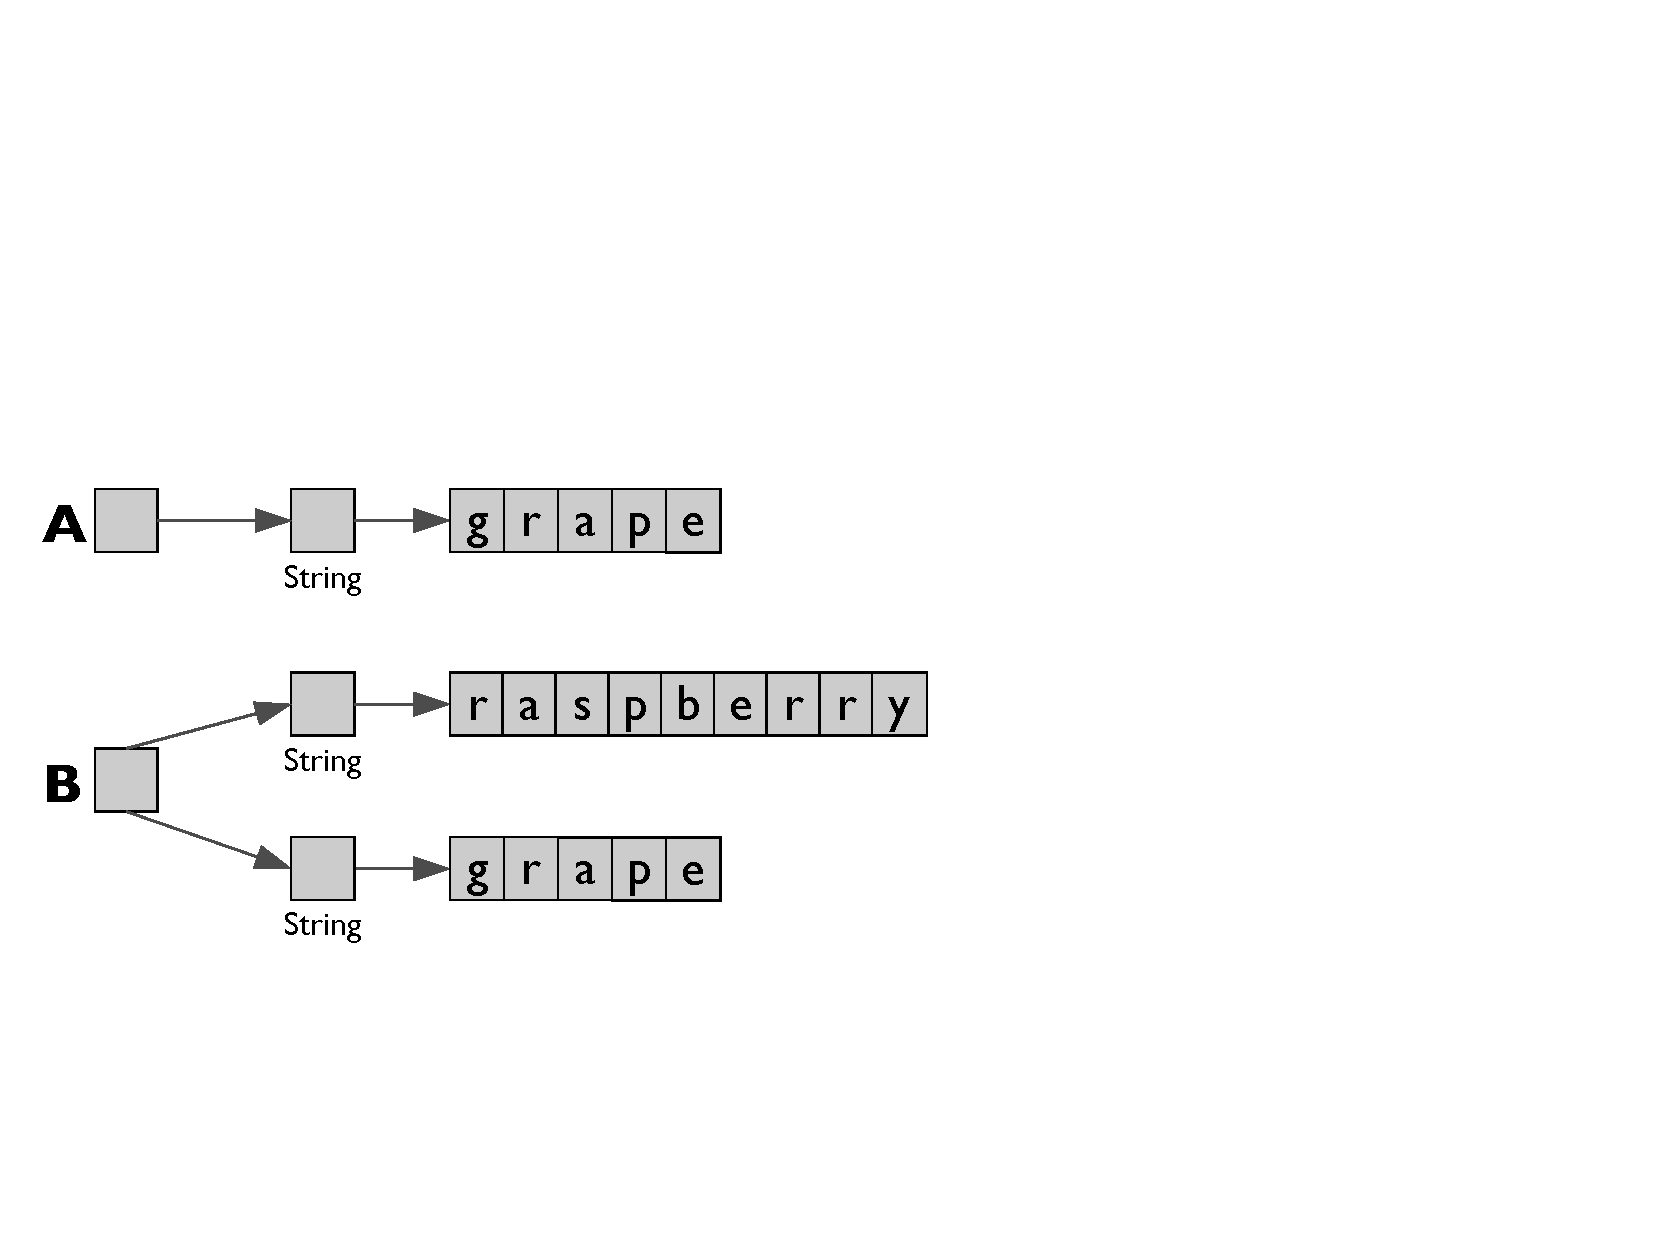
\includegraphics[width=0.425\textwidth]{part3/Figures/extreme/bulksharingpool1}}
	\qquad
	\subfigure[Interning.]{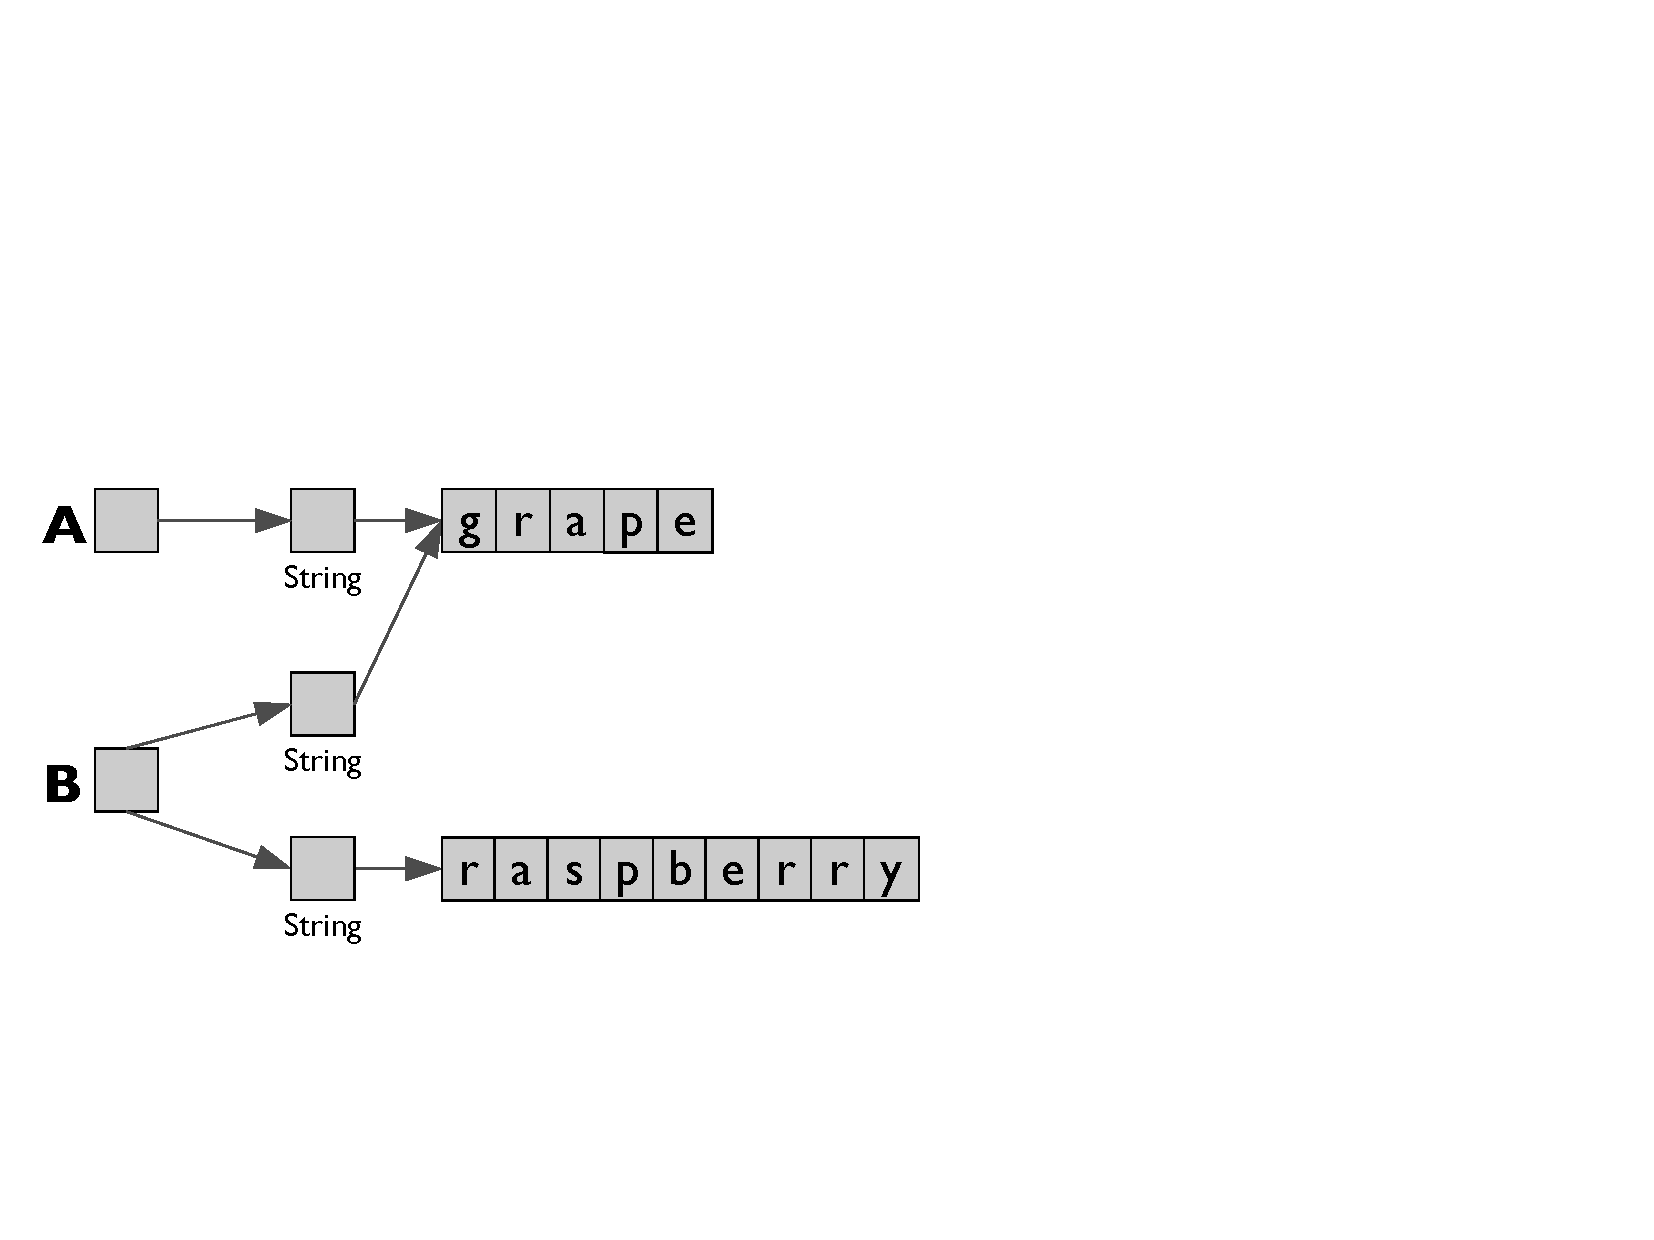
\includegraphics[width=0.425\textwidth]{part3/Figures/extreme/bulksharingpool2}}
	\qquad
	\subfigure[Bulk	sharing	pool.]{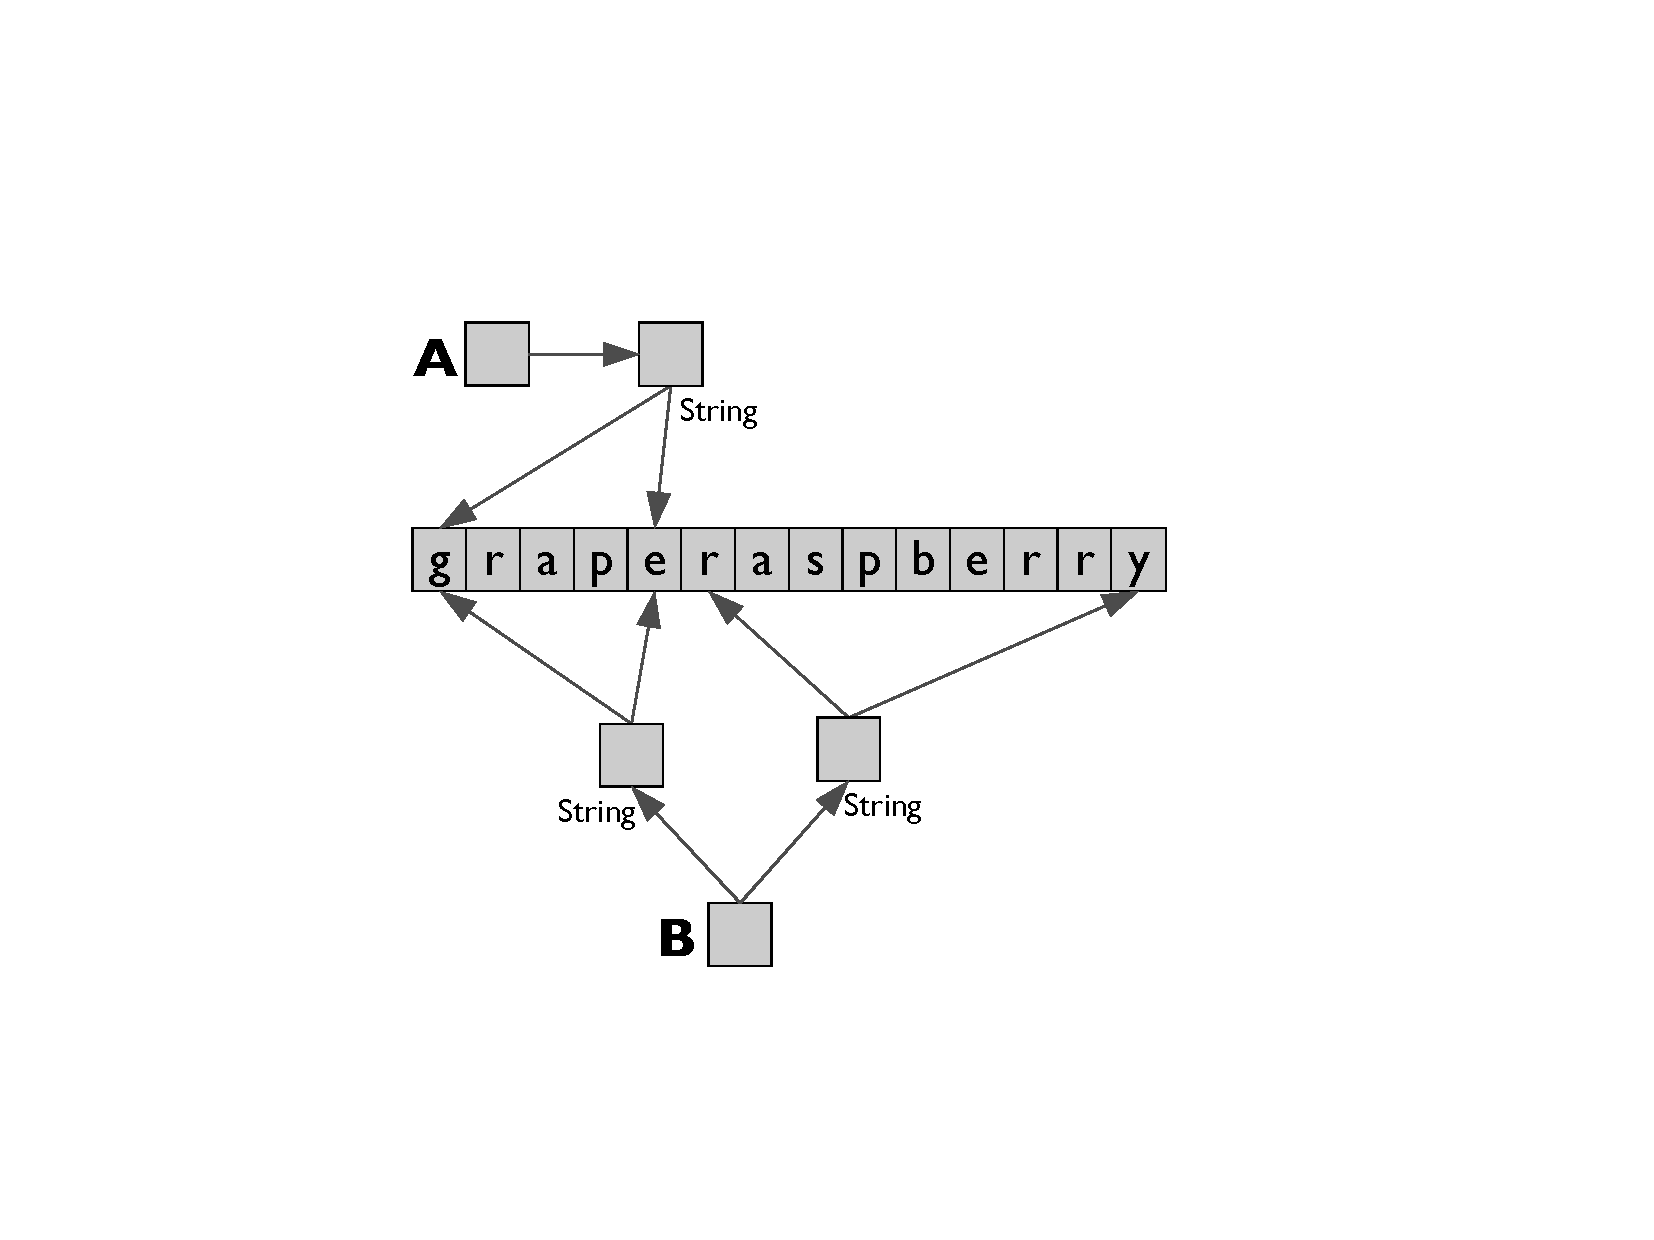
\includegraphics[width=0.36\textwidth]{part3/Figures/extreme/bulksharingpool3}}
	\qquad
	\subfigure[Bulk	sharing	pool, no wrappers.]{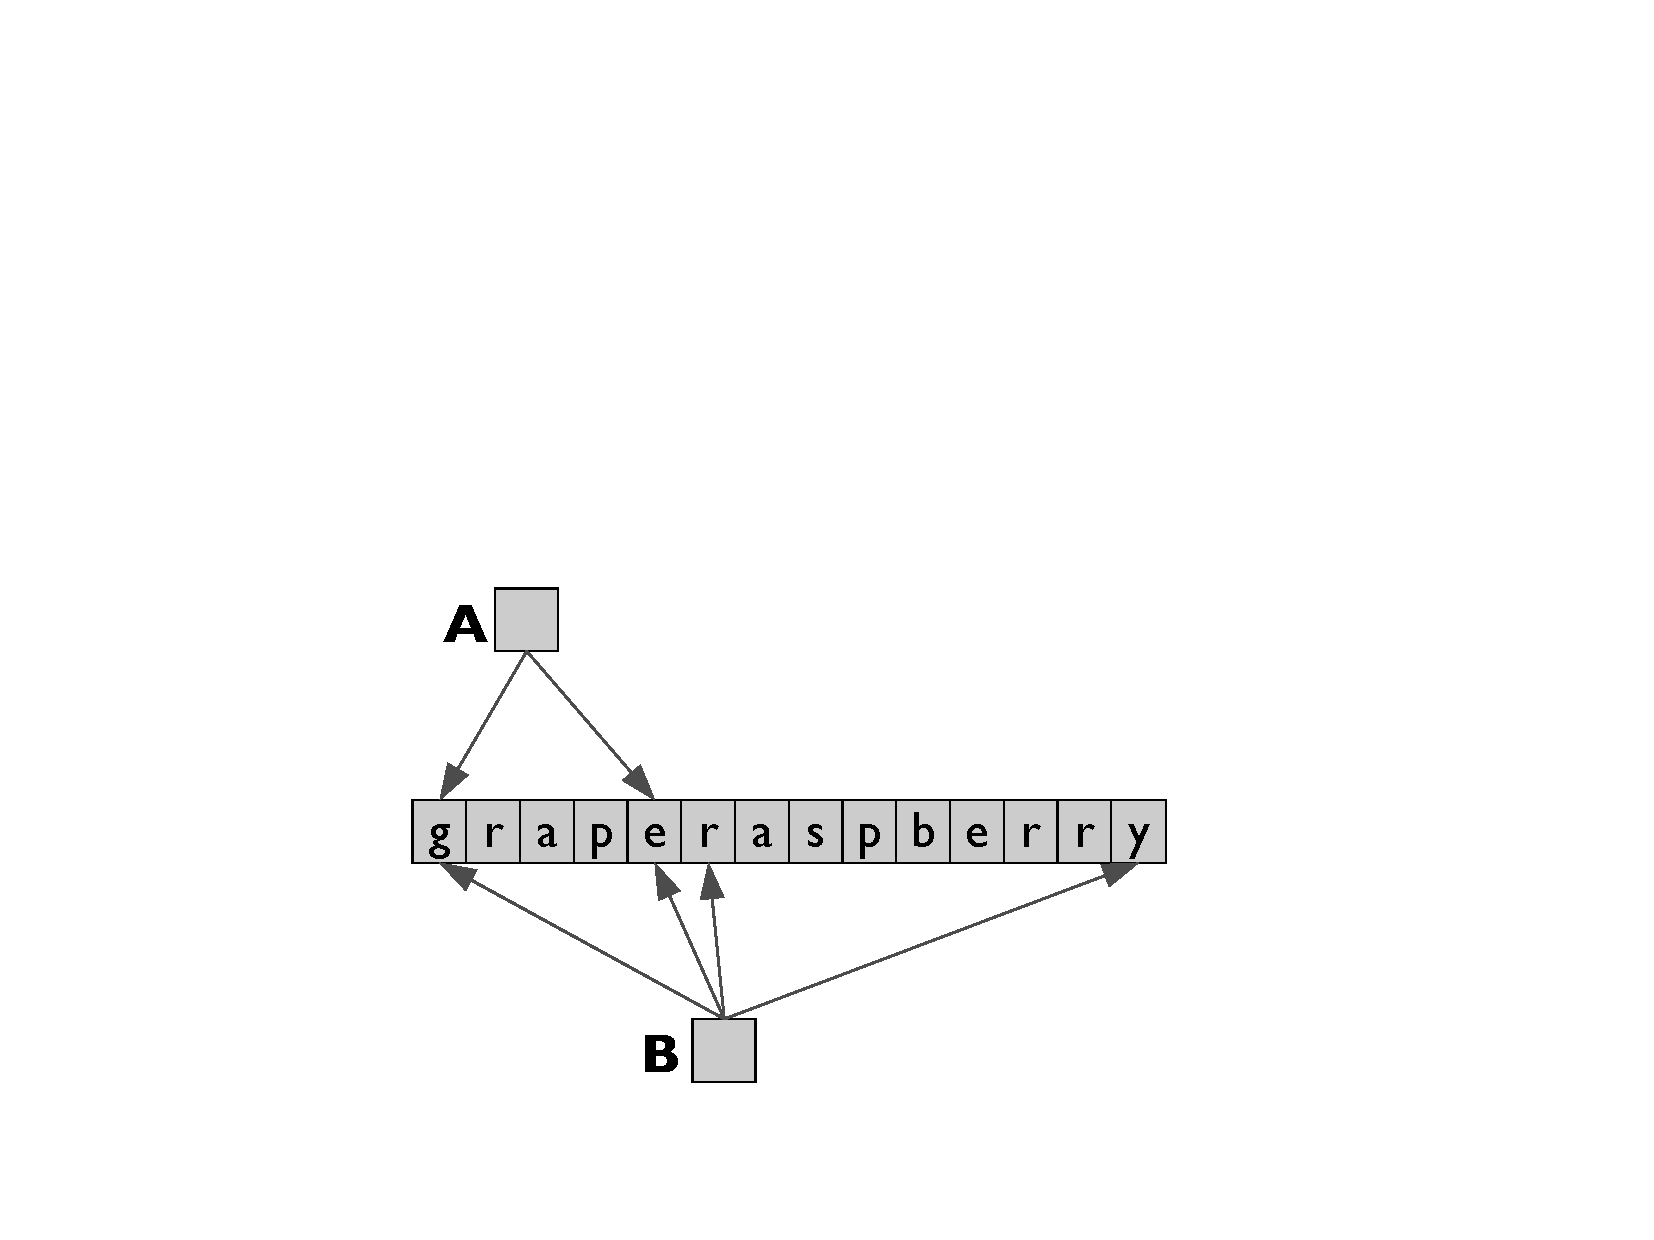
\includegraphics[width=0.36\textwidth]{part3/Figures/extreme/bulksharingpool4}}
	\subfigure[The memory consumed by one million strings, each of length 10
	bytes, for varying degrees degrees of distinctness; e.g. 10\% means that
	there are only 100,000 distinct strings.]{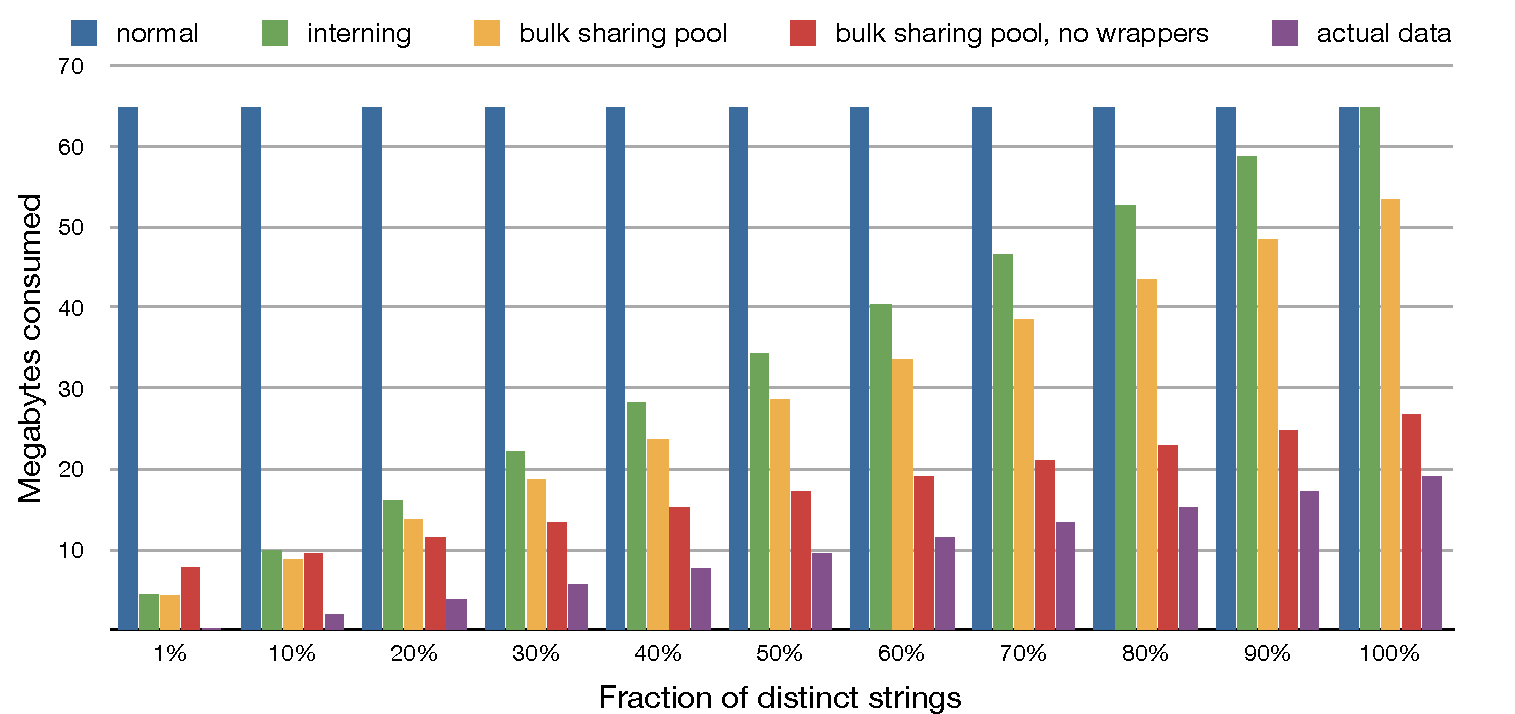
\includegraphics[width=\textwidth]{part3/Figures/extreme/bulksharingpool_consumptionchart.pdf}}
	\caption{If your application has many long-lived, but small, arrays of
	primitive data, it could suffer from high overhead. Interning avoids
	duplication. On top of interning, a Bulk Sharing Pool offers the additional
	potential for you to eliminate the primitive array wrappers, and so can be
	beneficial if there are still a large number of unique sequences.}
	\label{fig:bulk-sharing-pool}
\end{figure}

By eliminating many duplicates via interning, you stand to save a large amount of
memory, but your memory bloat factor will still be quite high. Instead of a bloat
factor of 83\%, with interning your heap will have a bloat factor of at least
88\%.
% 3*(16+32)/(10*2+3*(16+32))
This value is a lower bound, because there is another curious problem that arises
when handling duplicate data. If there is a bounded number of distinct sequences,
but an increasingly large number of total sequences, your memory bloat factor can
approach 100\%. In this case, the per-sequence memory overhead grows with the
number of sequences, but the amount of actual data is bounded by the number of
distinct sequences.

There are two further optimizations open to you, but these require deeper
changes. Both optimizations store all of the sequences in a single, large array.
This storage style is an example of optimizing for a bulk of uniformly typed data
that is accessed in a uniform, and stylized, fashion. Why pay the expense of many
small primitive arrays, if your code does not need each sequence to be a Java
object? If you will never synchronize or reflect on sequences, as objects, then
the primitive array header is a needless expense.
\autoref{fig:bulk-sharing-pool}(c) illustrates this bulk storage of the
sequences in a single large array. You pay the primitive array overhead just once, across
all pooled sequences, rather than for every sequence. 
%In this case, your heap
%will have a memory bloat factor of
% 3*(16+32)/(10*2+3*(16+32))

To achieve the ultimate in memory efficiency, you must also eliminate the
\class{String} wrapper objects, as shown in \autoref{fig:bulk-sharing-pool}(d).
This last step requires the most work on your part. If you have the luxury of
modifying the class definitions for the objects that contain the string
wrappers, then you can replace every pointer to a string with two numbers. These
numbers store indices into the single large array of bulk data, and demark the
sequence that the string wrapper would have contained. You are essentially
inlining the offset and length fields that every Java \class{String} object has,
and doing away with the hashcode field and the extra header and pointers. This
eliminates almost all sources of overhead.

This last, most extreme, optimization can reap large benefits in scalability,
but not always! You are paying an offset and length field in every object, even
when the strings are the same. For example, in
\autoref{fig:bulk-sharing-pool}(d), the offset and length fields for the two
uses of ``grape'' contain the same data. In the previous two optimizations,
these two fields are factored out into a separate \class{String} object, and so
only stored once. If the fraction of distinct strings
is small, then the cost of these duplicated fields outweighs the benefit of
removing the wrappers; it even outweighs the cost of removing the character
array headers. Where is the cross-over point?

\autoref{fig:bulk-sharing-pool}(e) shows the memory consumption of the four
implementations: using normal Java \class{Strings} without any attempt to remove
duplicates; using Java's built-in string interning mechiansm; using a bulk
sharing pool; and using a bulk sharing pool without any \class{String} wrappers.
The chart also includes a series comparison with the amount of memory consumed by
actual data.  The chart shows memory consumption of each implementation for
varying degrees of distinctness of the strings, for an case with one million
strings of length 10 characters each.
For example, if 500 thousand of the million strings are distinct (which
corresponds to the 50\% point in the chart), the normal implementation consumes
65 megabytes, the interning implementation consumes 34 megabytes, the bulk
sharing pool implementation consumes 27 megabytes, and the bulk implementation
without string wrappers consumes 17 megabytes. There are 500 thousand
distinct characters, so the actual data consumes about 10 megabytes. You can see
that the cross-over point, where the most extreme optimization begins to pay
off, occurs when about 10\% of the strings are distinct.

The chart makes it pretty clear how much a few headers and pointers can affect
the scalability of your application. With only a bit of work, you can have an
implementation that scales very well, with only minimal overhead on top of the
actual data.

\paragraph{Limitations of Bulk Storage Strategies}

There are two main problems you will run into, with a column-oriented approach.
The first has been touched on briefly: the lack of strong typing for nodes and
edges. If everything is just an integer, your code will be buggy and hard to
maintain. Java does not have a facility for naming types, such as \code{typedef}
in the C language. The Java \code{enum} construct seems like it could help, but
this use case would require a permanent object for every node, and, besides,
this construct is limited to around 65,000 entries per enumeration. You can use transient
nodes, with some cost to performance, but your code must still obey an implicit
contract, one not enforced by the \code{javac} compiler, that reference equality
is never used on these transient facades.

The second problem centers around modifications to the node or edge model. This
style of storage works fantasically well, much better than normal Java objects,
for certain kinds of modifications. Adding attributes to models is easy.
Adding nodes is straigtforward. However, deleting nodes, and adding or
removing edges from existing nodes can only be done with some extra work. For
deletions, you would have to implement a form of garbage collection yourself.
Nodes and edges can be marked as deleted; deleted elements would be ignored by
normal access mechanisms. Adding edges to existing nodes is even more difficult.
For these reasons, it is highly recommended that you only employ column-oriented
storage for data structures that do not change in these ways.


\section{Summary}




% Shortly, we will discuss the
%complexities, but benefits, of the latter style of API.

